\documentclass[12pt, a4paper]{article}
\usepackage{amsmath}
\usepackage{amsfonts}
\usepackage{amsthm}
\usepackage{mathtools}
\newtheorem{theorem}{Theorem}[section]
\newtheorem{definition}{Definition}[section]
\numberwithin{equation}{section}
\usepackage{pgfplots}
\pgfplotsset{width=10cm,compat=1.9}
\graphicspath{ {img/} }
\DeclareGraphicsExtensions{.png}

\title{Artificial Neural Networks}
\author{Kristian Wichmann}

\begin{document}
\maketitle

\section{Overview of artificial neural networks}
An \textit{artificial neural network} (ANN) superficially mimics the workings of the brain by being made up of \textit{neurons} and \textit{dendrites/axons}\footnote{In real neural networks, dendrites carry inputs to the neuron, while axons carry outputs from the neuron.}.

The neurons are organized into \textit{layers}. These come in three categories:
\begin{itemize}
\item The \textit{input layer}, into which data the data to be processed enters.
\item \textit{Hidden layers} - which are layers between the input and output layers.
\item The \textit{output layer} in which the result of the ANN's data processing can be read.
\end{itemize}

An ANN has at least three layer: Input, output and at least one hidden layer. An ANN with two or more hidden layers is known as a \textit{deep network}. 

Figure \ref{fig:ann_example} shows a neural network with three laters: 3 cells in the input layer, 4 cells in the hidden layer, and 2 cells in the output layer.

\begin{figure}
\centering
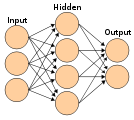
\includegraphics{artificial_neural_network}
\caption{An ANN with three layers.}
\label{fig:ann_example}
\end{figure}

The cells in each layer are connected by dendrites/axons, which are represented as arrows in figure \ref{fig:ann_example}: Every cell in each layer is connected to all the cells in the next layer.

As the data put into the input layer is translated into \textit{activity} levels in the cells. These activities then propagate via the axons through the network, causing different activity levels in each layer. The is repeated, until reaching the conclusion: The activity levels in the output layer. These are then interpreted accordingly.

\section{Mathematical formulation}

\subsection{Neuron activity}
The activity of a neuron is affected by all dendrites pointing to the cell, i.e. all cells in the previous layer. To compute the activity, all the inputs are weighted corresponding to the strength of each dendrite. In addition a \textit{bias} term may be added - a constant term.

The result is then put into an \textit{activation function} to yield the activity of the neuron.

Mathematically, this may be formulated:
\begin{equation}
\label{neuron_activity}
a_\textrm{neuron}=f\left(\sum_{i=1}^n \theta_i x_i + x_0\right)
\end{equation}
Here, $a$ is the activation, the $x_i$ are the inputs ($n$ total), the $\theta_i$ the corresponding weights (strength of the dendrites), $x_0$ is the bias term and finally $f$ is the activation function.

\begin{figure}
\centering
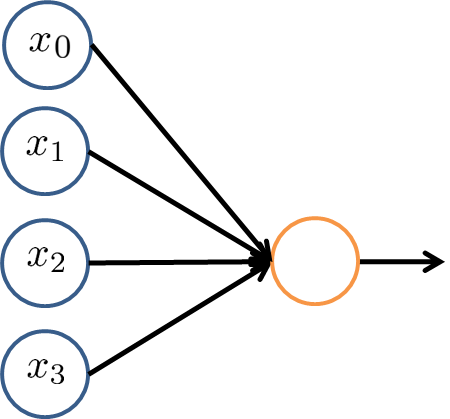
\includegraphics[width=50mm]{neuron}
\caption{Neuron with three inputs and a bias term}
\label{fig:neuron}
\end{figure}

The situation is outlined in figure \ref{fig:neuron}. Note that the bias has been shown as an input, even if this is not really the case: It is merely a constant term.

The inputs and weights are often written in vector form:
\begin{equation}
x=\begin{pmatrix}
x_1 \\ x_2 \\ \vdots \\ x_n
\end{pmatrix},
\quad
\theta=\begin{pmatrix}
\theta_1 \\ \theta_2 \\ \vdots \\ \theta_n
\end{pmatrix}
\end{equation}
Hence, equation \ref{neuron_activity} may be written:
\begin{equation}
a_\textrm{neuron}=f\left(\theta^T x + x_0\right)
\end{equation}

\subsection{Activation function}
For our activation function, we will choose the \textit{logistic function}. This is also known as the \textit{sigmoid function}\footnote{Though technically, any function with an s-shaped graph could be called a sigmoid function.}. It is defined as:
\begin{equation}
\label{sigmoid}
g(z)=\frac{1}{1+e^{-z}}
\end{equation}
The function is graphed in figure \ref{fig:sigmoid}. It can be though of as a "smoothed out step function"\footnote{A neuron with an actual step function as an activation function is known as a \textit{perceptron}.}.

\begin{figure}
\centering
\begin{tikzpicture}
\begin{axis}[
    axis lines = left,
    xlabel = $z$,
    ylabel = {Activation},
    ymin = 0,
    ymax = 1.2,
]
\addplot [
    domain=-6:6, 
    samples=50, 
    color=red,
]
{1/(1+exp(-x)};
\addlegendentry{$g(z)$}
\end{axis}
\end{tikzpicture}
\caption{The sigmoid function.}
\label{fig:sigmoid}
\end{figure}

The reason for the choice of this function is two-fold. First of all, it introduces \textit{activation saturation} into the model: Even if $\theta^T x+x_0$ turns out to be very large, the corresponding activity will still be close to 1. Similarly large negative values produce activities close to 0.

However, many functions could have achieved activation saturation. But $g(z)$ also has an additional nice mathematical property. Consider its derivative:
\begin{equation}
g'(z)=\frac{1'\cdot(1+e^{-z})-1\cdot(1+e^{-z})'}{(1+e^{-z})^2}=\frac{e^{-z}}{(1+e^{-z})^2}=\frac{e^{-z}}{1+e^{-z}}g(z)
\end{equation}
It turns out the first factor is equal to $1-g(z)$:
\begin{equation}
1-g(z)=1-\frac{1}{1+e^{-z}}=\frac{1+e^{-z}}{1+e^{-z}}-\frac{1}{1+e^{-z}}=\frac{1+e^{-z}-1}{1+e^{-z}}=\frac{e^{-z}}{1+e^{-z}}
\end{equation}
So we have:
\begin{equation}
\label{sigmoid_derivative}
g'(z)=g(z)\left(1-g(z)\right)
\end{equation}

\subsection{Matrix form of layer activities}
So, given cell number $i$ in layer $L$, its activation depends on the input activities from layer $L-1$, the activity is:
\begin{equation}
\label{layer_activity}
a^{(L)}_i=g\left(\left(\theta^{(L)}_i\right)^T a^{(L-1)} + b_i^{(L)}\right)
\end{equation}
Here, the activities from layer $L-1$ has been collected into the vector $a^{(L-1)}$ and the biases into the vector $b^{L}$. However, this may simply be expressed through matrix multiplication:
\begin{equation}
a^{(L)}=g\left(\theta^{(L)}a^{(L-1)}+b^{(L)}\right)
\end{equation}
Here, the matrix $\theta^{(L)}$ has rows consisting of weights for each cell. Also, $g$ is to be applied component-wise.

\subsubsection{Dimensionalities}
If layer $L-1$ contains $m_{L-1}$ cells and layer $L$ contains $m_L$ cells, this means the dimensionality of the matrices and vectors above are:
\begin{equation}
a^{(L-1)}\in\mathbb{R}^{m_{L-1}\times 1},\quad a^{(L)}, b^{(L)}\in\mathbb{R}^{m_L\times 1},\quad\theta^{(L)}\in\mathbb{R}^{m_L\times m_{L-1}} 
\end{equation}

\subsection{Output layer as a function of input layer}
If there is a total of $K$ layers in the ANN. Then the input layer is $x\equiv a^{(1)}$ and the output layer $y\equiv a^{(K)}$. Then we may express $y$ as a function of $x$ through repeated application of equation \ref{layer_activity}. This process is known as \textit{forward propagation}:
\begin{equation}
\label{hypothesis}
y=g\Bigg(\theta^{(K)}\bigg(\cdots g\Big(\theta^{(3)} g\big(\theta^{(2)}x+b^{(2)}\big)+b^{(3)}\Big)\cdots\bigg)+b^{(K)}\Bigg)\equiv h^{(\theta,b)}
\end{equation}
Here the notation $h_{\theta,b}(x)$ been introduced. Here $h$ stands for \textit{hypothesis}, i.e. the hypothesis that the particular choices of $\theta$ and $b$ are appropriate.

\section{ANN used for classification}
As an example, consider an ANN trained for picture classification. Se we imagine an ANN which has a representation of a picture for inputs $x$. The output layer is a series of $n$ numbers between 0 and 1. We may interpret these as probabilities. Maybe an ANN has been trained to recognize cats, dogs and horses. In this case, the size of the output layer is 3, and $y_1, y_2$ and $y_3$ are interpreted as the probabilities of the input picture containing a cat, dog or a horse respectively. If we know the picture only contains one animal, we would simply pick the highest value and use the corresponding animal as prediction.

\subsection{Training an ANN - overview}
So the question is now how to train an ANN for classification? This is a supervised machine learning problem, as we imagine we have a large dataset to train the network on.

The actual training is done using \textit{maximum likelihood estimation} of the weights and biases. In practice, this will be done using gradient or a similar optimization algorithm. The partial derivatives needed for this is found using what is known as the \textit{backpropagation algorithm}.

All of these topics will be the subject of the next set of sections.

\section{Likelihood of a Bernoulli process}
Let's take a step back and consider a Bernoulli process, i.e. an experiment with two outcomes: success and failure. The probability of success is called $p$, and hence the probability of failure must be $1-p$. This may be summed up in the equation:
\begin{equation}
P(x|p)=p^x(1-p)^{1-x},\quad x=0,1
\end{equation}
Here $x=1$ indicates success and $x=0$ failure.

The "probability mindset" here is, that if we know $p$ we know the distribution. The idea of likelihood swaps this around: Instead we ask what the parameter $p$ might be given the outcome $x$:
\begin{equation}
\mathcal{L}(p|x)=p^x(1-p)^{1-x}
\end{equation}
Based on the observation, we will then pick the value of $p$ that makes the observation most likely. This is known as maximum likelihood estimation\footnote{For a single observation this means the estimate is $p=1$ in case of success and $p=0$ in case of failure. In other words $p=x$.}.

Often, it is more convenient to minimize the \textit{log-likelihood}, i.e. minus the logarithm of the likelihood\footnote{Not all presentations include the minus sign. It is kept here to make $L$ a cost function.}. Since $\log$ is monotone, this is equivalent. For the Bernoulli process:
\begin{equation}
L(p|x)=-\log\mathcal{L}(p|x)=-x\log p-(1-x)\log(1-p)
\end{equation}
This can also be seen as a \textit{cost function}, i.e. something we wish to minimize. Figure \ref{fig:bernoulli} graphs the function for the two values of $x$.

\begin{figure}
\centering
\begin{tikzpicture}
\begin{axis}[
    axis lines = left,
    xlabel = $p$,
    ylabel = {Log-likelihood},
    ymin = 0,
    ymax = 2,
]
\addplot [
    domain=0:1, 
    samples=50, 
    color=red,
]
{-ln(x)};
\addlegendentry{$x=1$}

\addplot [
    domain=0:1, 
    samples=50, 
    color=green,
]
{-ln(1-x)};
\addlegendentry{$x=0$}

\end{axis}
\end{tikzpicture}
\caption{Log-likelihoods for the Bernoulli process.}
\label{fig:bernoulli}
\end{figure}

\section{Single item training set}
Now consider a single item training set, i.e. an input $x$ that has been classified as option $a$. This corresponds to a Bernoulli process for each cell in the output $y$, with only the $a$'th one being a success. So the desired output is $y=\delta_a$.

Now, the log-likelihood of the $i$'th such Bernoulli process depends on the actual choice of weights and biases - more specifically, it depends on the $h^{(\theta,b)}$ function defined in equation \ref{hypothesis}:
\begin{equation}
L_i(\theta,b|y_i)=-y_i\log\left[h^{(\theta,b)}_i\right]-(1-y_i)\log\left[1-h^{(\theta,b)}_i\right]
\end{equation}
If the processes are assumed to be independent (a big if, but let's go with that for now), the log-likelihoods add up, and the total likelihood is:
\begin{equation}
L(\theta,b|y)=\sum_i\left\{-y_i\log\left[h^{(\theta,b)}_i\right]-(1-y_i)\log\left[1-h^{(\theta,b)}_i\right]\right\}
\end{equation}
The task is now to find the weights and biases that minimize this. To do so, we wish to use gradient descent, and so need the partial derivatives of $L$ with respect to all weights and biases!

If $\alpha$ is any weight or bias, we can differentiate $L$ with respect to it:
\begin{equation}
\frac{\partial L}{\partial\alpha}=\sum_i\left\{-y_i\frac{1}{h^{(\theta,b)}_i}\frac{\partial h^{(\theta,b)}_i}{\partial\alpha}-(1-y_i)\frac{1}{1-h^{(\theta,b)}_i}\left(-\frac{\partial h^{(\theta,b)}_i}{\partial\alpha}\right)\right\}
\end{equation}
Collecting terms:
\begin{align}
\frac{\partial L}{\partial\alpha}=&\sum_i\left\{\frac{-y_i\left(1-h^{(\theta,b)}_i\right)+(1-y_1)h^{(\theta,b)}_i}{h^{(\theta,b)}_i(1-h^{(\theta,b)}_i)}\frac{\partial h^{(\theta,b)}_i}{\partial\alpha}\right\}\\
&\sum_i\left\{\frac{h^{(\theta,b)}_i-y_i}{h^{(\theta,b)}_i\left(1-h^{(\theta,b)}_i\right)}\frac{\partial h^{(\theta,b)}_i}{\partial\alpha}\right\}
\label{general_partial_formula}
\end{align}
So the problem is reduced to finding partial derivatives of $h$.

\subsection{Partial derivatives: Output layer}
The values of the output layer can be expressed through their dependence on the last hidden layer as per equation \ref{layer_activity}:
\begin{equation}
h^{(\theta,b)}=a^{(K)}=g(\theta^{(K)}a^{(K-1)}+b^{(K)})
\end{equation}
Remember that this is a vector equation - we need to consider each component. The property of the sigmoid function expressed in equation \ref{sigmoid_derivative} now comes in handy when we want to calculate partial derivatives:
\begin{equation}
\frac{\partial h^{(\theta,b)}_i}{\partial\alpha}=g(z_i)(1-g(z_i))\frac{\partial z_i}{\partial\alpha},\quad z_i=\sum_j\theta^{(K)}_{ij}a^{(K-1)}_j+b^{(K)}_i
\end{equation}
But $g(z_i)=h^{(\theta,b)}_i$! So inserting into equation \ref{general_partial_formula} there's a lot of cancellation:
\begin{equation}
\frac{\partial L}{\partial\alpha}=\sum_i\left\{\left(h^{(\theta,b)}_i-y_i\right)\frac{\partial z_i}{\partial\alpha}\right\}=\sum_i\delta^{(K)}_i\frac{\partial z_i}{\partial\alpha}
\label{general_partial_formula2}
\end{equation}
Here, the \textit{error} $\delta^{(K)}=h^{(\theta,b)}_i-y_i$ for the output layer has been introduced. This can be seen as the amount the hypothesis specified by the current weights and biases is off compared to what is desired. Be careful to distinguish between the error and Kronecker deltas in the following!

Equation \ref{general_partial_formula2} may be written in vector form:
\begin{equation}
\frac{\partial L}{\partial\alpha}=\left(\delta^{(K)}\right)^T\frac{\partial z}{\partial\alpha}
\end{equation}

Finally, we need to find the partial derivatives of $z$. Again, remember that $z$ is a vector:
\begin{equation}
z_i=\sum_j\theta^{(K)}_{ij}a^{(K-1)}_j+b^{(K)}_i
\end{equation}
At this point we only consider weights and biases from the axons pointing at the output layer, i.e. with superscript $K$. But since the weights form a matrix and the biases a vector, the resulting derivative objects will be 3 and 2-dimensional respectively:
\begin{equation}
\frac{\partial z_i}{\partial\theta^{(K)}_{kl}}=\sum_j\delta_{ik}\delta_{jl}a^{(K-1)}_j=\delta_{ik}a^{(K-1)}_l,\quad\frac{\partial z_i}{\partial b^{(K)}_k}=\delta_{ik}
\end{equation}
This means that the only non-zero derivatives are:
\begin{equation}
\frac{\partial z_i}{\partial\theta^{(K)}_{ij}}=a^{(K-1)}_j,\quad\frac{\partial z_i}{\partial b^{(K)}_i}=1
\end{equation}
We may now calculate the derivatives of $L$:
\begin{align}
\label{weight_derivative}
\frac{\partial L}{\partial\theta^{(K)}_{ij}}=&\sum_k\delta^{(K)}_k\delta_{ki}a^{(K-1)}_j=\delta^{(K)}_i a^{(K-1)}_j\\
\label{bias_derivative}
\frac{\partial L}{\partial b^{(K)}_i}=&\sum_k\delta^{(K)}_k\delta_{ki}=\delta^{(K)}_i
\end{align}

\subsection{Partial derivatives: Hidden layers}
On to the hidden layers. Luckily, it turns out that most of the calculations echo the output layer one closely.

Let's look at a weight or bias $\alpha$ from the last hidden layer. We need the derivative of $h$ with respect to $\alpha$. It is convenient to make the following definition:
\begin{equation}
z^{(N)}=\theta^{(N)}a^{(N-1)}+b^{(N)}
\end{equation}
Then we may write:
\begin{equation}
h^{(\theta,b)}=g(z^{(K)})
\end{equation}
Now we wish to form the partial derivative with respect to a weight/bias $\alpha$ from the last hidden layer, i.e. layer $K-1$. Here in vector form:
\begin{equation}
\frac{\partial h^{(\theta,b)}}{\partial\alpha}=g(z^{(K)})\odot(1-g(z^{(K)})\odot\frac{\partial z^{(K)}}{\partial\alpha}
\end{equation}
Here, the symbol $\odot$ is used to mean the \textit{Hadamard product} or \textit{Schur product}. It simply takes two vectors of equal length and return another vector of the same length, where each component is the product of the relevant factor components:
\begin{equation}
\begin{pmatrix}
a_1 \\ a_2 \\ \vdots \\ a_n
\end{pmatrix}
\odot
\begin{pmatrix}
b_1 \\ b_2 \\ \vdots \\ b_n
\end{pmatrix}
=
\begin{pmatrix}
a_1 b_1 \\ a_2 b_2 \\ \vdots \\ a_n b_n
\end{pmatrix}
\end{equation}
So what is the derivative? It is almost the same calculation as above:
\begin{equation}
\frac{\partial z^{(K)}}{\partial\alpha}=\frac{\partial}{\partial\alpha}g(z^{(K-1)})=g(z^{(K-1)})(1-g(z^{(K-1)}))\frac{\partial z^{(K-1)}}{\partial\alpha}
\end{equation}
Again, the two first factors can be expressed as activiations, and because $\alpha$ is associated with layer $K-1$, the derivative is analogous to the results from equations \ref{weight_derivative} and \ref{bias_derivative}. Inserting into equation \ref{general_partial_formula}, once again, there's some cancelling out, but this time we get some extra factors:
\begin{equation}
\frac{\partial L}{\partial\alpha}=\sum_i\left\{\delta^{(K)}_i a_i^{(K-1)}\left(1-a_i^{(K-1)}\right)\frac{\partial z^{(K-1)}_i}{\partial\alpha}\right\}
\end{equation}
Now, set the error of layer $K-1$ equal to:
\begin{equation}
\delta^{(K-1)}=\delta^{(K)}\odot a_i^{(K-1)}\odot\left(1-a^{(K-1)}\right)
\end{equation}
The calculations are now essentially the same as in the last section, and we get:
\begin{align}
\frac{\partial L}{\partial\theta^{(K-1)}_{ij}}=&\delta^{(K-1)}_i a^{(K-2)}_j\\
\frac{\partial L}{\partial b^{(K-1)}_i}=&\delta^{(K-1)}_i
\end{align}
If $\alpha$ had been associated with an earlier hidden layer, we could have followed the same steps iteratively, defining the error of layer $N$ recursively:
\begin{equation}
\delta^{(N)}=\delta^{(N+1)}\odot a_i^{(N)}\odot\left(1-a^{(N)}\right),\quad N\ge 2
\end{equation}
The general formulas for the derivatives is then:
\begin{align}
\frac{\partial L}{\partial\theta^{(N)}_{ij}}=&\delta^{(N)}_i a^{(N-1)}_j\\
\frac{\partial L}{\partial b^{(N)}_i}=&\delta^{(N)}_i
\end{align}
Again, $N$ should be at least 2, reflecting the fact that there's no error, weights or biases for the input layer.

\subsection{Backpropagation algorithm}
As we have seen above, calculation of derivatives is a recursive process, starting from the output layer and working backwars. Hence the name \textit{backpropagation algorithm}. Here are the steps in bullet form:
\begin{itemize}
\item First calculate all the activations of the neurons corresponding to the input $x$ and the current weights and biases.
\item Using the $y$'s, calculate the error of the output layer.
\item Repeat the following until all derivatives are calculated:
\begin{itemize}
\item Calculate derivatives for the current layer using the layer's error and the previousy calculated activations.
\item Iteratively calculate the error of the previous layer.
\end{itemize}
\end{itemize}
This is merely one step in the gradient descent process. The derivatives are used to generate a new set of weights/biases and the process is repeated until all derivatives are sufficiently small.

\section{Full training set}
So far, we've been dealing with the situation for a training set consisting of only one item. In practice, we ideally want to train our ANN on a large dataset.

However, since each item in the training set is independent of each other, the log-likelihood of multiple items is simply equal to the sum of all of them. By additivity of the derivative, the backpropagation process essentially remains the same, except we need to sum over the entire training set in each step of the gradient descent.

\end{document}